\section{Drones}
\subsection{Hello, photogrammetry-in-a-nutshell}
There are many scanning technologies, each with tradeoffs. There are two umbrella classes of scanning technologies: contact, and non-contact. The former relies on physical contact with the scanned object, and so is not applicable in this project. The latter may be either active or passive. Active solutions emit an electromagnetic wave, and based off its round-trip time, triangulated position, polarisation, or deformation of a rigid pattern, can detect the shape of the surface. Passive solutions merely record the scene under stereoscopic vision, different lighting conditions, or are reconstructed through computer vision. Photogrammetry---our weapon of choice---is reconstructed through computer vision, and has benefits through superior captured textures, capturing a photographic dataset usable by stonemasons for damage anaylsis, has no distance or size limitations, and can use relatively stock hardware.

Photogrammetry belongs to the field of \emph{structure from motion}, or \emph{SfM}. SfM takes a collection of photos as input, processes it, and outputs a 3D point cloud. The processing consists of three major steps: feature extraction, feature matching, and sparse bundle adjustment.  The first step identifies distinctive image features that may be common across multiple photographs. This uses the \emph{Scale-Invariant Feature Transform}, or SIFT method, which is an $O(N)$ algorithm, and may be parallelized. The second finds matching features between photos, in an $O(N^2)$ computation. Finally, 3D geometry is estimated from the matched features. This is also practically a $O(N^2)$ process. 

The final output from the photogrammetry process is a sparse point cloud. To make it more useful for visualisation, a dense reconstruction step then identifies likely surfaces. From this dense point cloud, the surface may be reconstructed, using a variety of surface reconstruction algorithms which provide a mesh-based output. Although the point cloud and their embedded RGB data is more ``accurate'' and contains enough colour to visualise the surface, the mesh-based output is desirable as it allows textures to be mapped onto it from the original photo collection. This UV-mapping process can be, and is automated. With an unbiased renderer providing lighting and autogenerated normal and occlusion maps, it can provide a very convincing reconstructed render.

\subsection{Drone flying tips}
A lot of common sense applies here: windy or rainy days are a bad idea. Oddly shaped surfaces (such as foliage) creates turbulence and dangerous flying areas. It is worthwhile to manually fly around the area during different wind conditions to get an intuitive idea of the potential issues. Flying with a spotter is very important.

\subsubsection{Scanning motions}
% TODO

\subsection{Upstream software documentation}
Nothing beats upstream documentation for authority.
\begin{description}
    \item[vsfm] \url{http://ccwu.me/vsfm/index.html}
    \item[siftgpu] \url{http://www.cs.unc.edu/~ccwu/siftgpu/manual.pdf}
    \item[bundler] \url{https://www.cs.cornell.edu/~snavely/bundler/bundler-v0.4-manual.html}
    \item[cmvs / pmvs2] \url{http://www.di.ens.fr/cmvs/documentation.html}
    \item[pmvs2] \url{http://www.di.ens.fr/pmvs/documentation.html}
    \item[pba] \url{http://grail.cs.washington.edu/projects/mcba/}
    \item[MeshLab] \url{http://meshlab.sourceforge.net/}
    \item[CloudCompare] \url{http://www.danielgm.net/cc/}
\end{description}
\subsection{Test cases}
A Utah teapot equivalent is very useful for testing the reconstruction process. Thankfully, {\tt pba} ({\tt Bundler}) includes two examples which are quick to execute: {\tt examples/ET} and {\tt examples/kermit}. For convenience, the kermit files have been included\footnote{{\tt src/kermit/*.jpg}}.

For reconstruction, the Standford Bunny and friends that live inside the Stanford 3D scanning repository\footnote{\url{http://graphics.stanford.edu/data/3Dscanrep/}} should be used.
\subsection{Scanning images}
The best image dataset for photogrammetry has a large (70\%) overlap, has an image sequence that shows an incrementally changing viewpoint, and has textured surfaces with lots of unique feature points.

It is impractical to manually capture photos of a large and complex object. A more practical approach is either continuous burst photography or video. The former is preferred, as photographs usually have a higher quality than a video, unless RAW video is possible with the camera.

If video is used, the frames may be extracted easily with {\tt ffmpeg}\footnote{\url{https://www.ffmpeg.org/}}:

\begin{lstlisting}
$ ffmpeg -i /path/to/input.video -r 2 -f image2 -start_number 0 image-%07d.jpg
\end{lstlisting}

The {\tt -start\_number} argument makes it convenient to append image sequences from multiple videos. Note that the {\tt .jpg} extension is required for processing by {\tt vsfm}. If image quality issues occur from the JPG encoding, the {\tt -q} argument may be used, or instead bypassed by exporting to {\tt .ppm}.

Additional format conversions are trivially done with {\tt mogrify} from {\tt imagemagick}.

\subsection{Non-headless execution}

Non-headless execution is trivial and documented on the vsfm homepage.

\subsection{Headless execution}
The {\tt VisualSFM} documentation\footnote{{\tt \url{http://ccwu.me/vsfm/doc.html}}} and {\tt -h} argument describes the command parameters quite well. In explicit terms, the {\tt sfm} argument invokes headless execution. Additional arguments are appended for the matching process, sparse reconstruction process, and dense reconstruction process, in that order (with some additional options for fine-tuning). An example which performs all processes would be:
\begin{lstlisting}
$ VisualSFM sfm+pmvs /path/to/jpgs/ /path/to/output.nvm
\end{lstlisting}
When processing large datasets, execution should be batched, and resumable if it fails. Let's say we are merely interested in the matching process, and it terminates before it has finished:
\begin{lstlisting}
$ VisualSFM sfm+skipsfm /path/to/jpgs/^C^C^C
# Now, resume. All steps may be resumed in a similar manner.
$ VisualSFM sfm+skipsfm /path/to/jpgs/
\end{lstlisting}
Matching results in {\tt *.sift} and {\tt *.mat} files to store the results. Now that matching is complete, sparse reconstruction can begin. Reconstruction results are stored in a {\tt .nvm} file.
\begin{lstlisting}
$ VisualSFM sfm /path/to/jpgs/ /path/to/output.nvm
\end{lstlisting}
And once sparse reconstruction is complete, we can do the dense reconstruction.
\begin{lstlisting}
$ VisualSFM sfm+loadnvm+pmvs /path/to/output.nvm /path/to/dense.nvm
\end{lstlisting}
This may be accompanied with the {\tt +subset} argument without any implications.
If the dataset is particularly large, it may be desirable to break up the first step into a separate sift (which generates {\tt .sift} files) and matching (which generates {\tt .mat} files) step.
\begin{lstlisting}
$ find . -type f -iname "*.jpg" > photos.txt
$ VisualSFM siftgpu photos.txt
$ VisualSFM sfm+skipsfm ./
\end{lstlisting}
\subsection{Execution times}
Processing is not fast. Specifically, a rigorous dataset of a couple thousand images will already take up multiple days\footnote{\url{https://groups.google.com/forum/\#!topic/vsfm/PegIJ0M0JaE}}. More images are better than less, with non-diminishing gains in reconstruction quality with an increase in the dataset. Before any further optimisations are made, it is important to make sure that the hardware ideally uses SiftGPU, rather than a CPU-based implementation, and uses multi-threaded matching and bundling. VisualSFM provides these features out of the box. A detailed analysis of VisualSFM's approach compared with a cluster based approach is described elsewhere\footnote{\url{http://ieee-hpec.org/2012/index\_htm\_files/Sawyer\_rev.pdf}}.

\begin{figure}[h]
\begin{center}
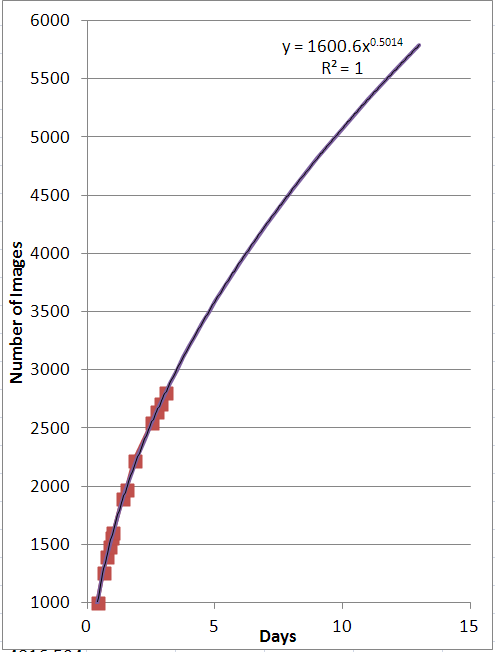
\includegraphics[width=6cm]{siftgpu_processing_times}
\caption{SiftGPU processing times on a CUDA-enabled Geoforce 660}
\end{center}
\end{figure}

\subsubsection{Preemptive feature matching}

A major bottleneck is the $O(N^2)$ image matching process. A solution is a one-time sort of the dataset into subsets to be matched, called \emph{preemtive feature matching}. Changchang Wu has documented the approach\footnote{\url{http://ccwu.me/vsfm/vsfm.pdf}}. By applying it, at the sacrifice of potential diminishing returns of output resolution, the image matching turns into a $O(N)$ process. The {\tt +subset} argument of {\tt VisualSFM} enables this feature, and can be applied mid-way through an execution.

\begin{lstlisting}
$ VisualSFM sfm+subset+skipsfm /path/to/jpgs/ /path/to/output.nvm
\end{lstlisting}

\subsubsection{Manual execution of dense reconstruction}

Note that this section does not apply for CMP+MVS reconstruction, where the process is significantly different.

{\tt vsfm} does not offer a very detailed breakdown of the dense reconstruction process, which has implications for batching and distributing jobs to a cluster. The dense reconstruction step also has quite a few parameters which may significantly affect execuation time. Although these may be edited in {\tt nv.ini}, they are unlikely to be globally appropriate, and so manual execution of each step is desirable. Finally, there are some options which are simply not exposed, or we would like to iterate through manually to optimise the results.

The dense reconstruction is broken down into 4 steps: {\tt cmvs} preparation, {\tt cmvs}, {\tt genOption}, and {\tt pmvs2}. {\tt cmvs} preparation selects the appropriate matched photos for {\tt cmvs} to execute, performs lens undistortion, and creates the necessary ascii input files. The inputs, processes, and outputs of the subsequent three steps are documented in their respective documentation, and so will not be elaborated here.

We can piggy-back on {\tt vsfm} to generate the appropriate input for {\tt cmvs}. This is an $O(N)$ CPU-intensive process. Once prepared, we can kill the {\tt vsfm} process, and any rogue {\tt cmvs} processes, and proceed manually.

\begin{lstlisting}
$ VisualSFM sfm+loadnvm+cmvs sparse.nvm dense.nvm
[ ... snip ... ]
# images loaded:     n
Load NVM for dense reconstruction
Save to ./dense.nvm ... done
Undistorting n images in model #n
[ ... snip ... ]
^C^C^C
\end{lstlisting}

The index of images to undistort are provided in {\tt dense.nvm.cmvs/00/list.txt}, so we can easily check to see how many images we are expecting, and whether or not we have finished undistorting all images:

\begin{lstlisting}
$ test -e $(echo $(tail -n 1 list.txt) | sed -e 's/\\/\//g' -e 's/://') && echo "yes" || echo "no"
\end{lstlisting}

Once complete, the {\tt dense.nvm.cmvs/00/} directory holds the formatted {\tt bundle.rd.out} file required for {\tt cmvs} to run. The {\tt cmvs} step is a memory intensive process. Even though it is possible to skip directly to the {\tt pmvs2} step, {\tt cmvs} should be executed first, as it provides clusters for {\tt pmvs2} to execute in parallel.

Nevertheless, {\tt cmvs} can still be daunting task for very large datasets. The memory usage depends primarily on the filtered photo collection in {\tt dense.nvm.cmvs/00/visualize/}. Once loaded into memory, it will start generating clusters. There are two parameters for this process: {\tt maximage} max images for the clusters, and {\tt CPU} number of CPUs or cores in the processing machine.

Although the {\tt cmvs} documentation stresses the {\tt maximage} parameter for controlling memory, a much more significant impact on memory usage can be made by modifying the source images. This is because all source images must be loaded for {\tt cmvs} to calculate the clusters. However, {\tt cmvs} does not simply cluster images blindly\footnote{\url{http://www.cse.wustl.edu/~furukawa/papers/cvpr10.pdf}}. Clustering both determines image neighbours, and following that, cluster neighbours, and additionally filters low resolution geometry. Modifications on the source would have an impact on the latter, but this may be acceptable if the clustering at least makes processing possible.

Let's say we have a memory limit, and we are feeling frisky.

\begin{lstlisting}
$ cp -r ./dense.nvm.cmvs/00/visualize ./dense.nvm.cmvs/00/visualise_highres
$ cd ./dense.nvm.cmvs/00/visualize/
$ mogrify -resize 50% "*.jpg"
\end{lstlisting}

Once memory restrictions are solved, we can proceed. However, {\tt maximage} affects the cluster size, and therefore can result in a (seemingly) infinite loop if a value that is too small is selected\footnote{\url{https://groups.google.com/forum/\#!topic/vsfm/Iq-ET0wwsdQ}}. A dumb but valid technique is to attempt as small an integer $n$ as possible above 1, and if a timeout is reached, attempt again with $n+1$. Starting with $n=5$, as used by {\tt vsfm} seems sensible.

\begin{lstlisting}
$ cmvs ./dense.nvm.cmvs/00/ 5 8
\end{lstlisting}

Once complete, {\tt genOption} can parse the {\tt ske.dat} to create the {\tt option-\%04d} files for {\tt pmvs2}. There are far more parameters for this process, and are documented with {\tt pmvs2}. It is encouraged to use the default values by the documentation, not the ones by {\tt vsfm}, and change the third argument, {\tt level} if resource limits are hit. As this is merely a parsing step, execution of the following command will be fast, but has implications with {\tt pmvs2}.

\begin{lstlisting}
$ genOption ./dense.nvm.cmvs/00/ 1 2 0.7 7 3 8
\end{lstlisting}

Depending on the number of {\tt option-\%04d} created, the jobs may then be queued to the cluster. If frisky memory management was applied, now is the time to backtrack our resolutions, as the smaller quantity of images per cluster means that memory should no longer be an issue.

\begin{lstlisting}
$ mv ./dense.nvm.cmvs/00/visualize ./dense.nvm.cmvs/00/visualise_lowres
$ mv ./dense.nvm.cmvs/00/visualize_highres ./dense.nvm.cmvs/00/visualise
\end{lstlisting}

Now it's just a matter of processing the job queue with {\tt pmvs2}.

\begin{lstlisting}
$ pmvs2 ./dense.nvm.cmvs/00/ option-0000
\end{lstlisting}

For testing without a cluster at hand, we have to do it all ourselves.

\begin{lstlisting}
#!/bin/bash
for f in ./dense.nvm.cmvs/00/option-*
do
    name=`basename $f`
    pmvs2 ./dense.nvm.cmvs/00/ $name
done
\end{lstlisting}

\subsubsection{Structured sequences}

Planning out reconstructions through \emph{structured sequences} can bypass much of the clustering that {\tt cmvs} provides. There are senarios where this is necessary. For example, downsampling the images may not be acceptable for the {\tt cmvs} step. Or perhaps the structure is far too complex and needs such a large dataset that would take too long to process atomically.

In this scenario, essentially the clustering that {\tt cmvs} provides will be done manually. The building must be scanned in portions, and reconstructed in portions, and finally stitched together. When doing this, stitching may be problematic.

There are two stitching strategies: pre-surface reconstruction, and post-surface reconstruction.
% TODO

\subsection{Headless environment}
Although {\tt VisualSFM} can be run headlessly, the package has dependencies on a graphics card, some X libraries, and an OpenGL environment. Cheap virtualised hardware---such as Linode---is inappropriate. A CPU-only matching and sparse reconstruction has been tested on a Linode environment, but is not documented here, and nor is it worth pursuing.
\subsubsection{Sandbox environment}
A Gentoo system is recommended due to the rather bleeding edge condition of the packages and pipeline. This gives us a replicatable vanilla environment that supports and encourages compilation from source. Test setups were done in a {\tt chroot}.

Although the {\tt chroot} may be left as an exercise to the reader\footnote{\url{https://wiki.gentoo.org/wiki/Handbook:Main\_Page}}, a standard setup for a stage3 installation is shown:

\begin{lstlisting}
# Location of the chroot
$ mkdir ./stone
# Note that hardened stage3's have not been tested
$ links https://www.gentoo.org/downloads/mirrors/
$ tar xvjpf stage3-*.tar.bz2 -C ./stone/
$ cp /etc/resolv.conf ./stone/etc

# This mount process should be packaged for convenience
$ mount -t proc proc ./stone/proc
$ mount --rbind /sys ./stone/sys
$ mount --make-rslave ./stone/sys
$ mount --rbind /dev ./stone/dev
$ mount --make-rslave ./stone/dev

# Speak, friend, and enter ...
$ chroot ./stone /bin/bash

# Once inside ...
$ env-update
$ emerge-webrsync
$ emerge --sync
\end{lstlisting}

For completeness, we also unmount when finished:

\begin{lstlisting}
$ umount -l ./stone/dev{/shm,/pts,}
$ umount ./stone{/boot,/sys,/proc,}
\end{lstlisting}
\subsubsection{Alternative environments}
As a quick detour, I'd like to mention alternative black box environments that may help in testing.

A detailed vanilla compilation guide is provided for a Ubuntu 12.04 environment\footnote{\url{http://www.10flow.com/2012/08/15/building-visualsfm-on-ubuntu-12-04-precise-pangolin-desktop-64-bit/}}. It is worthwhile reading to gain an understanding of the dependencies and their build process.

Additionally, there is also ArcheOS\footnote{\url{http://www.archeos.eu/}}, a Debian-based distribution meant for archaeologists. It bundles other useful utilities, including the Python Photogrammetry Toolkit (PPT) which may be of interest if there are licencing issues with vsfm.
\subsubsection{Basic package compilation and dependencies}
Portage, as expected, does not keep vsfm and friends in the main tree. The {\tt cg} overlay provides the related packages.

\begin{lstlisting}
$ emerge -av layman
$ echo "source /var/lib/layman/make.conf" >> /etc/portage/make.conf
$ layman -L
$ layman -a cg
\end{lstlisting}

There is the usual barrage of keywords, uninteresting USE-flags, and licensing.

\begin{lstlisting}
$ mkdir /etc/portage/package.keywords
$ touch /etc/portage/package.keywords/vsfm
$ echo "=media-gfx/PoissonRecon-6.13 ~amd64" >> /etc/portage/package.keywords/vsfm
$ echo "=media-libs/graclus-1.2 ~amd64" >> /etc/portage/package.keywords/vsfm
$ echo "=media-libs/pba-1.0.5 ~amd64" >> /etc/portage/package.keywords/vsfm
$ echo "=media-gfx/pmvs-2-r1 ~amd64" >> /etc/portage/package.keywords/vsfm
$ echo "=sci-libs/cminpack-1.3.4 ~amd64" >> /etc/portage/package.keywords/vsfm
$ echo "=media-gfx/vsfm-0.5.26 ~amd64" >> /etc/portage/package.keywords/vsfm
$ echo "=media-gfx/siftgpu-0.5.400-r1 ~amd64" >> /etc/portage/package.keywords/vsfm

$ touch /etc/portage/package.use/vsfm
$ echo "media-gfx/siftgpu cuda" >> /etc/portage/package.use/vsfm
$ echo "x11-drivers/nvidia-drivers gtk2" >> /etc/portage/package.use/vsfm

$ mkdir /etc/portage/package.license
$ touch /etc/portage/package.license/vsfm
$ echo "dev-util/nvidia-cuda-toolkit NVIDIA-CUDA" >> /etc/portage/package.license/vsfm
\end{lstlisting}

Note the {\tt media-gfx/siftgpu cuda} above, as this assumes a CUDA environment, and all the 32-bit/64-bit issues and updated graphics drivers that come with it. Resolving this is an exercise for the reader.

In addition to the regular dependencies resolved by portage, {\tt media-gfx/vsfm} requires {\tt x11-libs/libXext} and {\tt media-libs/freeglut}. These should be emerged before {\tt media-gfx/vsfm}.

\begin{lstlisting}
$ emerge -av libXext freeglut vsfm
\end{lstlisting}

Once compiled, vsfm expects to find sift in {\tt ./sift}. Unfortunately, the packaged binary is named differently. This is a simple fix:
\begin{lstlisting}
$ ln -s /usr/bin/SimpleSIFT /usr/bin/sift
\end{lstlisting}

\subsubsection{Using CPU-based sift for a non-CUDA environment}
Once SIFT is found, matching and sparse reconstruction should work out of the box. However, if the environment does not have a CUDA-capable GPU, switching to CPU for sift may be necessary. This requires editing the {\tt nv.ini} file, which is generated upon the first run of {\tt VisualSFM}. Once run, it may be found in the counter-intuitive location of {\tt /usr/bin/nv.ini}. It should be modified so that {\tt param\_use\_siftgpu 0} is set. The configuration is heavily documented inline for more information.

Now that {\tt VisualSFM} is searching for a CPU implementation of sift, we have the choice to use either Lowe's SIFT or VLFeat SIFT instead of SiftGPU\footnote{\url{http://ccwu.me/vsfm/doc.html\#download\_urls}}. Lowe's SIFT is already packaged including binaries, and so it is a simple matter to download it, and replace the previous symlink in {\tt /usr/bin/sift} to point to Lowe's SIFT.

\subsubsection{Patching CMVS and PMVS}
Once matching and sparse reconstruction is working, there may still be issues with {\tt cmvs} and {\tt pmvs2}. Gentoo's {\tt media-gfx/pmvs} is incomplete in that it only provides the {\tt pmvs2} binary, and not {\tt cmvs}. Although {\tt media-gfx/cmvs} seems to provide the necessary binaries, they have a bug which I have elaborated upon\footnote{\url{https://groups.google.com/forum/embed/\#!topic/vsfm/QKZ9MbTKpeE}}, but not yet figured out an appropriate patch for the overlay.

The solution is to compile pmvs2 manually. However, we can still reuse the {\tt cmvs} binary provided by the overlay. The explicit steps (to be executed with due diligence) are shown:

\begin{lstlisting}
# Let's make use of the overlay as much as possible
$ emerge -av media-gfx/cmvs
# Notice this is not pmvs-2-fix0.tar.gz
$ wget http://www.di.ens.fr/pmvs/pmvs-2.tar.gz
# lapack is a dependency for manual compilation
$ emerge -av virtual/lapack
$ tar -xzvf pmvs-2.tar.gz
$ cd pmvs-2/program/main
$ cp mylapack.o mylapack.o.backup
$ make clean
$ cp mylapack.o.backup mylapack.o
$ make depend
$ make
$ mv /usr/bin/pmvs2 /usr/bin/pmvs2-portage
$ ln -s /path/to/pmvs-2/program/main/pmvs2 /usr/bin/pmvs2
\end{lstlisting}

\subsubsection{Job queues and synchronisation}

With a headless setup needing to process many buildings throughout the year, it makes sense to elaborate on synchronising datasets/results to/from the client/server. A ~4200 photo dataset, with 3840x2160px dimensions has a total size of ~1.2GB. This illustrates the practicality of transferring over datasets to remote hosts.

The transfer process should be done securely, robustly, and explicitly one-way. {\tt rsync} over {\tt ssh} is a natural solution, with potential automation with {\tt lsyncd} (not documented here, but trivial to implement).

\begin{lstlisting}
$ rsync -avz /path/to/dataset/ user@host:/path/to/processor/inbox
\end{lstlisting}

% TODO rabbit
\subsection{Point cloud realignment}

The generated point cloud has an arbitrary direction and scale. We need to realign the point cloud using datum points based off a master template for each building site. The master template can be a point cloud scan that is arbitrarily chosen with an arbitrary location, rotation, and scale. All that matters is that subsequent scans, supporting models, polyhedron bounds, or supplementary material have a way to align themselves to match this chosen datum.

The realignment is a two step process, executed with {\tt CloudCompare}. First is a rough alignment, the two clouds are roughly placed in the same location, rotation, and scale. This is done through specifying a minimum of 4 datum points on the slave model, then their corresponding datum points on the master model, and aligning them. Then, a precise alignment is performed using cloud registration where the computer will iteratively optimise the position to minimise errors. It is recommended to allow the scale to be adjusted during this process, as photogrammetry reconstructions do not share scale.

Upon doing either of these two steps, a calculated transformation matrix is returned by {\tt CloudCompare}, which may be logged for future use in scripts. As the rough alignment is a visual process, there is little value is headlessly running this step.

\subsection{Point cloud cleaning}

Before the model is useful for visualisation or surface reconstruction, it is important to clean up the point cloud first. Nonsensical points and points unrelated to the scanned object should be removed. This is a visual process, and may be non-trivial to do manually, depending on the site. For example, dust, clouds, specular materials, camera artifacts, or simply poor computer vision can result in patches of clearly incorrect point clouds.

\subsubsection{Manual cleaning}
Depending on the surface reconstruction process that is planned, there are two approaches to manual cleaning. If a large amount of point metadata should be maintained (e.g. point normals, as required for poisson reconstruction), the cleaning should be done with a program that retains this, such as {\tt Meshlab}. Alternatively, {\tt CloudCompare} offers more sophisticated selection tools. If this is not required, any 3D modeling suite, such as {\tt Blender} would be more appropriate, as it offers much more convenient mesh selection tools. It should be noted that a modeling suite may not be able to render vertex colours, if they are not part of a face, and so may make it much harder to visualise what you are cleaning. Of course, it is possible to use both.

The actual process of selecting and deleting points is trivial, and not documented here.

\subsubsection{Automated cleaning}

When dealing with messy clouds, cleaning can be a tedious process. In some cases, where the object is concave in all axes, manual cleaning becomes impossible, due to the 2D projection used in the software's selection tools. Using 3D bounding boxes or other forms of cutting planes are inappropriate for any marginally complex building form. Specifically, the problem is difficult in that the errant points may be quite close to a valid surface, and the surface may also be concave.

The problem may be solved by creating a low-poly bounding polyhedron template for each building site, and using a ``point-in-polyhedron'' algorithm\footnote{\url{http://erich.realtimerendering.com/ptinpoly/}} that supports concave surfaces. This is the same as a ``point-in-polygon'' algorithmn except that axes are intelligently discarded for the test. Each point in the cloud can then be tested against the boundary. If the point lies outside the boundary, it is discarded.

No known software is available that provides this polyhedron containment functionality with any form of usable interface. We will therefore write our own. One library that provides an implementation of this polyhedron test is {\tt MathGeoLib}\footnote{\url{http://clb.demon.fi/MathGeoLib/nightly/}}. Let's compile it:

\begin{lstlisting}
$ git clone https://github.com/juj/MathGeoLib.git
$ cd MathGeoLib
$ cmake
$ make
\end{lstlisting}

Now we have the linkable static library {\tt libMathGeoLib.a}. Now we will need to deal with two meshes: the point cloud and the bounding mesh (assuming both have been aligned to the datums properly). We can parse the {\tt .ply} format for this.

The {\tt .ply} format\footnote{\url{http://people.cs.kuleuven.be/~ares.lagae/libply/ply-0.1/doc/PLY_FILES.txt}} is chosen to process for multiple reasons: it is the output of {\tt pmvs2}, it is simple to parse, it explicitly supports custom metadata in the case of future customisation, it is the standard supported by the Standford benchmark, and originally designed for 3D scanning.

The chosen {\tt .ply} parser is {\tt libply}\footnote{\url{http://people.cs.kuleuven.be/~ares.lagae/libply/}}. If {\tt gcc} 4.2.0 is not available to compile it, I have patched it to compile it with 4.9.3, and included the patch with this document\footnote{{\tt src/libply.patch}}. Now we can compile it:

\begin{lstlisting}
$ wget http://people.cs.kuleuven.be/~ares.lagae/libply/ply-0.1.tar.gz
$ tar -xzvf ply-0.1.tar.gz
$ cd ply-0.1/
$ ./configure --prefix=/home/foobar
$ make
$ make install
\end{lstlisting}

Note the location of the installed library files, as they will be needed to compile our point cloud cleaner.

It should be noted that the {\tt .ply} parsing (and other functions) library used by {\tt MeshLab} is VCG\footnote{\url{http://vcg.isti.cnr.it/vcglib/index.html}}. It may be beneficial to rewrite the parser using VCG to minimise file handling quirks. Usage of VCG is apparently straightforward with the inclusion of their header files (no apparent static or shared libraries), but I was unable to get the PLY importer headers to compile smoothly, probably due to the cygwin environment. If it is rewritten with VCG, their import class supports all major mesh file formats.

Now that dependencies are resolved, we can compile our homebrew {\tt point\_cloud\_cleaner}. The source has been included with this document\footnote{{\tt src/point\_cloud\_cleaner.cpp}}. It's straightforward to compile:

\begin{lstlisting}
$ g++ point_cloud_cleaner.cpp -L/path/to/libply/static/lib -lply -L/path/to/MathGeoLib -lMathGeoLib -I/path/to/ply-0.1 -I/path/to/MathGeoLib/src -o point_cloud_cleaner
\end{lstlisting}

And equally simple to run:

\begin{lstlisting}
$ point_cloud_cleaner boundary.ply cloud.ply output.ply
\end{lstlisting}

Note that {\tt boundary.ply} should be a triangulated mesh, as triangles are assumed within the code, and non triangles encourage non-coplanar faces, which have unpredictable results. Also, all {\tt .ply} formats should of the ASCII variant.

As the {\tt point\_cloud\_cleaner} is merely to parse the {\tt .ply} and execute the polyhedron containment test, formatting details of the output {\t .ply} are incomplete (and even wrong, if you have played with {\tt --format}). As such, instead of exorcising more C++, I have left cleaning the resultant {\tt .ply} files to {\tt sed}. As we're probably processing a whole group of meshes, it's a simple matter to contain everything in a {\tt bash} loop:

\begin{lstlisting}
#!/bin/bash
for f in ./src/option-*
do
    name=`basename $f`
    point_cloud_cleaner boundary.ply src/$name dest/$name
    sed -i '1,/ply/d' dest/$name
    sed -i '1s/^/ply\n/' dest/$name
    sed -i '/DEL/d' dest/$name
    VERTNUM=$(expr $(wc -l < dest/$name) - 13)
    sed -i "s/element vertex .*/element vertex $VERTNUM/" dest/$name
done
\end{lstlisting}

The process is not perfect, but executes with $O(N)$ and has few outliers.

\subsubsection{Automated cleaning optimisations}

It should be noted that a convex hull test is much more computationally efficient. Similarly, the boundary test depends on both the number of faces in the bounding polyhedron and the number of points in the point cloud. If the need arises, there should be multiple passes: a roughing pass that uses convex hulls, and then a more detailed pass.

Alternatively, the concave bounding polyhedron may be converted into a series of platonic solids\footnote{\url{http://paulbourke.net/geometry/platonic/}} (regular, convex polyhedra) which are then tested using convex algorithms. This could be done through Delaunay tetrahedralization\footnote{\url{http://wias-berlin.de/software/tetgen/}}. This approach has not been tested.

\subsection{Surface reconstruction}
As described, mesh output is usually desirable. Depending on the resolution and reliability of the point cloud, different surface reconstruction techniques may provide better results. The method recommended (and documented) here is \emph{Poisson surface reconstruction}. However, other reconstruction methods have been tested with varying results, and an understanding of the fundamental concepts of reconstruction are vital when things go sour.

There are two categories of surface reconstruction algorithms: \emph{computation geometry}, and \emph{implicit surfaces}. The former fits the mesh onto the points (such as \emph{Ball pivoting}), and the latter fits implicit functions (such as \emph{Poisson}), which are then solved using marching cubes. The challenges they face are how to deal with noisy point clouds. Noise in point clouds may be misplaced or offset points, non-uniform sampling or density, and gaps in the cloud. Some in the computation geometry category simply ignore gaps, or blindly connect all points, errant or not, and so require additional smoothing and blending steps. Some in the implicit surfaces category consider the points as a whole, and are able to stitch gaps, or ignore points that deviant from the main surface gradient, which may result in a smoother, but perhaps less accurate mesh.

As such, there is no single solution, but there is a general approach for surface reconstruction. After basic cleaning of the point cloud is done, additional cleaning may be necessary to prepare it for surface reconstruction. This may involve converting the cloud into a uniform density, reconstructing new normals, or smoothing existing point normals. Finally, the mesh is reconstructed---where apart from minor parameter tweaking is relatively simple with an established algorithm. A benchmark for different surface reconstruction techniques is available\footnote{\url{http://www.cs.utah.edu/~bergerm/recon_bench/}}.

\subsubsection{Poisson surface reconstruction}
Poisson surface reconstruction is a popular implicit surface algorithm. It is based off the Poisson equation, and the details are elaborated in the original paper\footnote{\url{http://research.microsoft.com/en-us/um/people/hoppe/poissonrecon.pdf}} by Microsoft. It is the de-facto reconstruction method for reliable point clouds which represent closed objects.

{\tt MeshLab} provides all the functionality required to perform this. First, we should resample the point cloud into a uniform density. This can be accomplished with \emph{Poisson-disk sampling}. \emph{Base Mesh Subsampling} is required as the point cloud only has vertices to work with instead of faces. A number of samples similar to the vertex count in the point cloud should be chosen, so that resolution is not lost.

Once the point cloud is clean, we can perform the Poisson surface reconstruction. The \emph{Octree Depth} changes the resolution of the implicit functions, which lead to higher resolutions, and so should be maximised\footnote{Oddly enough, 14 seems to be the max value}. Other values are less important, but may require tweaking if the mesh resolution or smoothness is not satisfactory, and are well documented in-program.

\subsubsection{Headless reconstruction and cleaning}

{\tt MeshLab} provides {\tt meshlabserver}, which can parse plaintext XML-based instructions headlessly. These instructions are called ``filter scripts'', and are generated by {\tt MeshLab}. It is trivial to manipulate the parameters programmatically for the server.

\subsection{Texture mapping}
To help visualise the scanned object, it is useful to have colour data. There are two sources of colour data: the sampled RGB data of the point cloud, or the original photos from the photogrammetry.
% TODO
\subsubsection{Vertex painting}
Vertex painting uses the point cloud RGB data as a source and applies the colours as a vertex paint to the mesh. Naturally, this uses much less memory as no rasters are required, however requires a much higher mesh resolution to look decent, and will lack the subtlety of a mapped texture. It is also very easy.

First, the dense point cloud(s) and the reconstructed mesh are loaded in {\tt MeshLab}. The mesh resolution will need to be increased, ideally to the same density as the point cloud. As the point cloud is rarely uniform there will be a mismatch of densities, and inefficiency of the mesh, but this is the sacrifice for ease of colouring. A \emph{Subdivision surface: Catmull-clark} should be applied with an appropriate number of iterations to achieve the density required.

Finally, a \emph{Vertex attribute transfer} should be applied to transfer the colour of the vertices to the target mesh. The max search distance should be minimised to avoid needless ``splotching'' of colours. Note that merging point cloud layers through {\tt MeshLab} does not retain colour data, so vertex attributes would be transferred one a layer by layer basis, or else we should manually merge layers (suspected to be trivial). This means that layer layers may override the details of original layers. With many layers this can be quite tiresome, and should be automated with a filter script.

\subsubsection{UV mapped textures}

Unless you're a fan of pointillism, you probably should go for UV mapped textures. Unfortunately, this process is very CPU and memory heavy.

\subsubsection{Axis mappings between formats}
% TODO

\subsection{Point cloud diffs}
It is perhaps useful to analyse the diffs between two point clouds to detect worn down elements or elements of the building that have simply disappeared.
% TODO


